\documentclass{article}
\usepackage{a4wide}
\usepackage{graphicx}

\begin{document}

\begin{titlepage}
    \begin{center}
        \textbf{\huge Earth GUI Plug-in Development Documentation}
    \end{center}
\end{titlepage}

\tableofcontents
\listoffigures
\newpage

\section{Introduction} % (fold)

Plugins are already existent in the Earth's daemon. However, this project had identified that this is a potential improvement towards the front-end. Thus, the concept of plugins for Earth's daemon was ported to the front-end. However, the concept needed some changes in order to make them work. 

Instead of following the daemon plugins' standards, the plugins for the front-end, dubbed as GUI plugins, were developed based on the Rails' plugin framework. The reason is to allow an easy to access portal to create, update and maintain these GUI plugins. Another reason why the Rails plugin framework was chosen is because Earth was built using the Rails web-application framework. 

The following section will present how do these plugins work in Models, Controllers and Views. Then, the rest of the sections will present how the plugins can be created and deployed.

% (end)

\section{Investigation} % (fold)

It was observed that it is better to make the front-end as plug-able as the daemon, so that users can easily add or remove GUI related functionalities. The problem with GUI plugins is that these plugins may not be as simple as the plugins created for the daemon. Their content, or rather codes, can be scattered over the three sections of the Rails development paradigm, which are the Models, Controllers and Views. However, the Rails plugin framework solves the problem. 

A Rails plugin is either an extension or a modification of the core framework. Such plugins can do almost anything that a Rails application can, plus a little more. The provider plugin \texttt{generator} script is able to copy the respective files into their respective \texttt{app} sub-directories. In addition, the \texttt{generator} script can process an \texttt{ERB} file and have it copied into the \texttt{migration} folder through the use of the following migration templates:

\begin{itemize}
    \item{\textbf{Models}} Put a model in the plugin’s \texttt{lib} folder and use \texttt{generator} to copy it to \texttt{app/models} folder.
    \item{\textbf{View Helpers}} A helper method can be included, or mixed, into the rest of the application. (This is also known as ``mixin''.) 
    \item{\textbf{Controllers}} Copies a controller into the \texttt{app/controllers} directory. 
    \item{\textbf{rake Tasks}} Creates a \texttt{rake} file into the tasks folder.
    \item{\textbf{Images, Stylesheets, Javascripts}} The \texttt{generator} copies these into the public directory.
    \item{\textbf{Test assertions}} To be mixed-in to the tests cases.
    \item{\textbf{Unit and Functional tests}} Can be generated like controllers.
\end{itemize}

From the investigation above, it is clear that the Rails plugin framework can be used to create Earth GUI plugins.

% (end)

\section{Preparation} % (fold)

To create a GUI plugin, one first needs to know what feature or functionality one wants to add, and how the result should be presented on the front-end. To do so, one needs to create necessary files in a directory of their preference. Then, one will need to have these plugin files copied into the \texttt{plugin} directory. Finally, use the \texttt{generator} script to process and copy the files into the Earth's \texttt{app} directory. The following sections will discuss the mentioned steps in detailed.

% (end)

\section{Implementation} % (fold)

The GUI plugin is implemented using the Rails plugin framework. However, some code changes were needed in the original View codes. This is to allow addition functionality, such as more tag or search field, to be added. The Rails plugin framework is used for the rest of the MVC model. The structure of the GUI plugin framework is shown Figure \ref{fig:flow}.

\begin{figure}[ht]
    \centering
    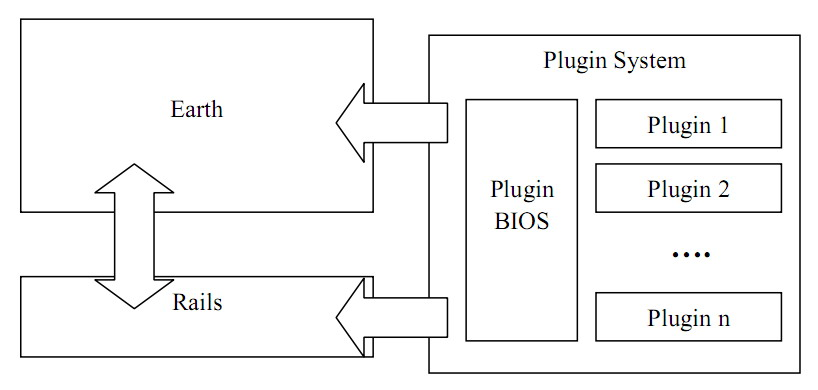
\includegraphics[scale=0.5]{fig/flow.jpg}
    \caption{The structure of the GUI plugin framework.}
    \label{fig:flow}
\end{figure}

Rails plugin framework can be used as an extension add more functionality development in Earth. It is helpful for development of Earth. In the  Plugin System, the Plugin BIOS was created. It is an intermediary communication layer between the plugins, Earth and Rails. Currently, this layer is only a simple communication layer. It is expected in the future this layer will be extended to include dependance checks and have features to have sub-classing ability. Each plugin, a configuration file named ``plugin\_cfg'' is created. This file contains the information about the plugin to be used as a manifest of the plugin package. 

% (end)

\section{Instruction} % (fold)

In this section, the steps of how to develop, install and uninstall a GUI plugin is presented. To ease explanation, a blank plugin, called ``mr\_bogus'', is used as an example. To begin, Figure \ref{fig:instruction-1} shows the original Earth front-end, before mr\_bogus is installed. 

\begin{figure}
    \centering
    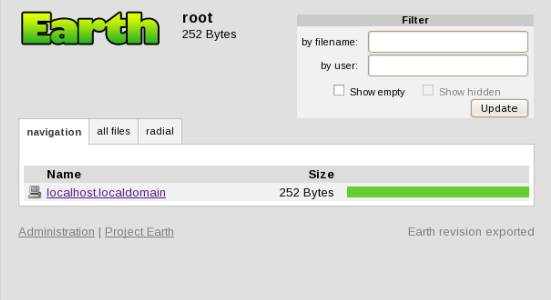
\includegraphics[scale=0.7]{fig/instruction-1.jpg}
    \caption{Original Earth front-end.}
    \label{fig:instruction-1}
\end{figure}

% (end)

\subsection{Development} % (fold)

As mentioned before, the \texttt{generate} script is first executed to create some basic necessary structures and files. To do so, the following command can be used:

\begin{verbatim}
    ./script/generate plugin mr_bogus --with generator
\end{verbatim}

\begin{figure}
    \centering
    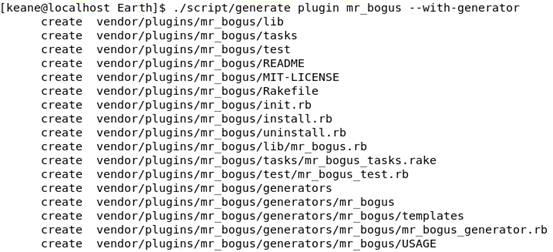
\includegraphics[scale=0.7]{fig/instruction-2.jpg}
    \caption{Running the \texttt{generate} script to create mr\_bogus plugin.}
    \label{fig:instruction-2}
\end{figure}

A blank plugin in Rails have been created after the previous command was executed successfully. At this stage, one can safely edit the affected files to have the final results displayed. Views can be added by creating new directories and files in the \texttt{./vendor/plugins/mr\_bogus/generators/ mr\_bogus/templates} directory. For example, the action controller needs the directory called ``controllers''. Finally, update the file called ``mr\_bogus\_generator.rb'', which can be executed to create particular file wherever one wants. More instructions can be found in this web-site \texttt{http://wiki.rubyonrails.com/rails/pages/HowTosPlugins}.

Here an action controller and a webpage were created for views:

\begin{verbatim}
    ./vendor/plugins/mr_bogus/generators/mr_bogus/templates/controllers/bogus_controller.rb
    ./vendor/plugins/mr_bogus/generators/mr_bogus/templates/views/bogus.rhtml
\end{verbatim}

Figure \ref{fig:instruction-3} shows the content of the \texttt{bogus\_controller.rb} file, and Figure \ref{fig:instruction-4} shows the content of the \texttt{bogus.rhtml} file.

\begin{figure}
    \centering
    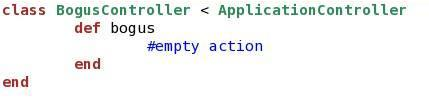
\includegraphics[scale=0.7]{fig/instruction-3.jpg}
    \caption{The \texttt{bogus\_controller.rb} file.}
    \label{fig:instruction-3}
\end{figure}

\begin{figure}
    \centering
    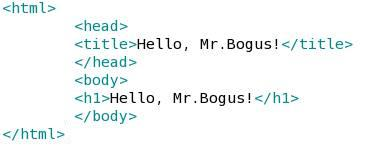
\includegraphics[scale=0.7]{fig/instruction-4.jpg}
    \caption{The \texttt{bogus.rhtml} file.}
    \label{fig:instruction-4}
\end{figure}

The file named \texttt{mr\_bogus\_generator.rb} would be modified for preparation of moving files to particular folders, as shown in Figure \ref{fig:instruction-5}.

\begin{figure}
    \centering
    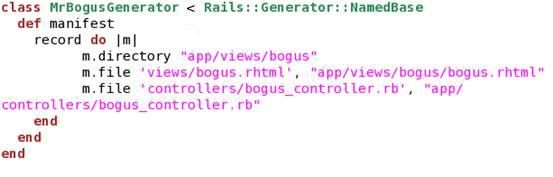
\includegraphics[scale=0.7]{fig/instruction-5.jpg}
    \caption{The \texttt{bogus\_controller.rb} file.}
    \label{fig:instruction-5}
\end{figure}

Once done, the following command can be executed to have the plugin implemented into Rails: 

\begin{verbatim}
    ./script/generator mr_bogus bogus
\end{verbatim}

To test the plugin, simply point the web-browser of choice to the following URL:

\begin{verbatim}
    http://localhost:3000/bogus/bogus
\end{verbatim}

However, the plugin should be implemented into the existing Earth system instead. To do so, a configuration file has to be created. The file is named ``plugin\_cfg'' in the \texttt{./vendor/plugins/mr\_bogus} directory. Figure \ref{fig:asd} shows the content of the configuration file.

\begin{figure}
    \centering
    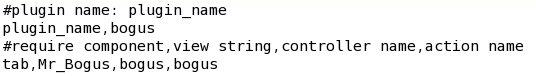
\includegraphics[scale=0.7]{fig/asd.jpg}
    \caption{The \texttt{plugin\_cfg} file.}
    \label{fig:asd}
\end{figure}

Now, point the web-browser to the homepage of Earth. The result is shown in Figure \ref{fig:instruction-6}. Figure \ref{fig:instruction-7} shows the implementation of the plugin.

\begin{figure}
    \centering
    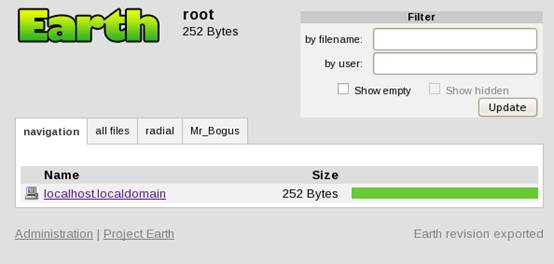
\includegraphics[scale=0.7]{fig/instruction-6.jpg}
    \caption{\texttt{mr\_bogus} implemented in Earth.}
    \label{fig:instruction-6}
\end{figure}

\begin{figure}
    \centering
    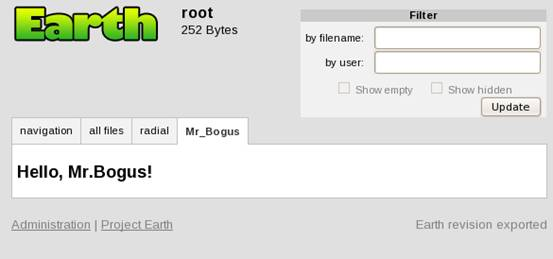
\includegraphics[scale=0.7]{fig/instruction-7.jpg}
    \caption{The \texttt{mr\_bogus} tab.}
    \label{fig:instruction-7}
\end{figure}

So far, the plugin had included a new tab in Earth. However, to add a new text field in the filter section, the following can statements can be added into the configuration file:

\begin{verbatim}
    #require componenet, view string, parameter name
    field_tag, by wine, wine
    field_tag, by cake, cake
\end{verbatim}

Figure \ref{fig:instruction-9} shows the refreshed the homepage of Earth.

\begin{figure}
    \centering
    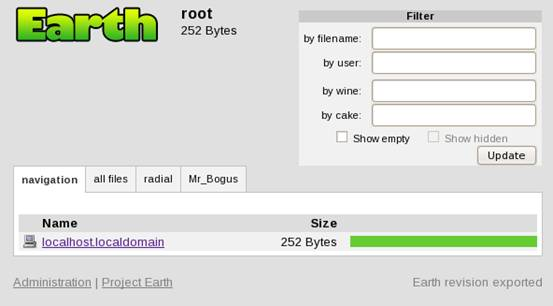
\includegraphics[scale=0.7]{fig/instruction-9.jpg}
    \caption{New text fields.}
    \label{fig:instruction-9}
\end{figure}

The plugin can now be tested and debugged. Finally, a set of installation and uninstallation scripts can be created from the following steps:

\begin{enumerate}
    \item Find files and folders created.
    \item Modify the installation in root of plugin to have the appropriate files copied to their appropriate destination directories.
    \item Build the plugin as a package including the installation file.
\end{enumerate}

The following is the content of installation of ``mr\_bogus'' named ``install.rb'':

\begin{verbatim}
    require 'fileutils' 
    plugin_name = ARGV[1] #mr_bogus 
    earth_root = ARGV[0]  
    puts "Creating the plugin" 
    system "ruby #{earth_root}/script/generate plugin #{plugin_name} --with-generator" 
    RAILS_ROOT = earth_root 
    FileUtils.cp File.join(File.dirname(__FILE__), 'init.rb'),File.join
    (RAILS_ROOT, 'vendor','plugins',plugin_name,'init.rb')  
    FileUtils.cp File.join(File.dirname(__FILE__), 'install.rb'),File.join
    (RAILS_ROOT, 'vendor','plugins',plugin_name,'install.rb')  
    FileUtils.cp File.join(File.dirname(__FILE__), 'uninstall.rb'),File.join
    (RAILS_ROOT, 'vendor','plugins',plugin_name,'uninstall.rb')  
    FileUtils.cp File.join(File.dirname(__FILE__), 'plugin_cfg'),File.join
    (RAILS_ROOT, 'vendor','plugins',plugin_name,'plugin_cfg') 
    FileUtils.cp File.join(File.dirname(__FILE__),'lib','mr_bogus.rb'),File.join
    (RAILS_ROOT, 'vendor','plugins',plugin_name,'lib','mr_bogus.rb')  
    FileUtils.cp File.join(File.dirname(__FILE__),'generators',plugin_name,
    'mr_bogus_generator.rb'),File.join(RAILS_ROOT,'vendor','plugins',plugin_name,
    'generators',plugin_name,'mr_bogus_generator.rb')  
    Dir.mkdir("#{RAILS_ROOT}/vendor/plugins/mr_bogus/generators/mr_bogus
    /templates/controllers") unless File.directory?("#{RAILS_ROOT}/vendor/plugins
    /mr_bogus/generators/mr_bogus/templates/controllers") 
    Dir.mkdir("#{RAILS_ROOT}/vendor/plugins/mr_bogus/generators/mr_bogus
    /templates/views") unless File.directory?("#{RAILS_ROOT}/vendor/plugins/mr_bogus/generators
    /mr_bogus/templates/views") 
    FileUtils.cp File.join(File.dirname(__FILE__),'generators',plugin_name,'templates',
    'controllers','bogus_controller.rb'),File.join(RAILS\_ROOT,'vendor','plugins',
    plugin_name,'generators',plugin_name,'templates','controllers','bogus_controller.rb') 
    FileUtils.cp File.join(File.dirname(__FILE__),'generators',plugin_name,'templates','views',
    'bogus.rhtml'),File.join(RAILS_ROOT,'vendor','plugins',plugin_name,'generators',
    plugin_name,'templates','views','bogus.rhtml') 
\end{verbatim}

An uninstallation file named ``uninstall.rb'' for removing the plugin created. Here is an example:\\

\begin{verbatim}
    require 'fileutils' 
    plugin_name = ARGV[1] #mr_bogus 
    earth_root = ARGV[0]  
    puts "Uninstalling the generator" 
    system "ruby #{earth_root}/script/destroy #{plugin_name} #{plugin_name}" 
    puts "Uninstalling the plugin" 
    system "ruby #{earth_root}/script/destroy plugin #{plugin_name} --with-generator" 
    system "rm -r #{earth_root}/vendor/plugins/#{plugin_name}"
\end{verbatim}

% (end)

\subsection{Installation} % (fold)

To install and activate the plugin, simply execute the following commands:

\begin{verbatim}
    ruby install.rb <root_earth> <plugin_name>
    ruby <root_earth>/script/generate <plugin_name> <plugin_name>
\end{verbatim}

% (end)

\subsection{Uninstallation} % (fold)

To uninstall, execute the following command:

\begin{verbatim}
    ruby uninstall.rb <root_earth> <plugin_name>
\end{verbatim}

% (end)

\end{document}
